\begin{figure}[H]
	\centering
	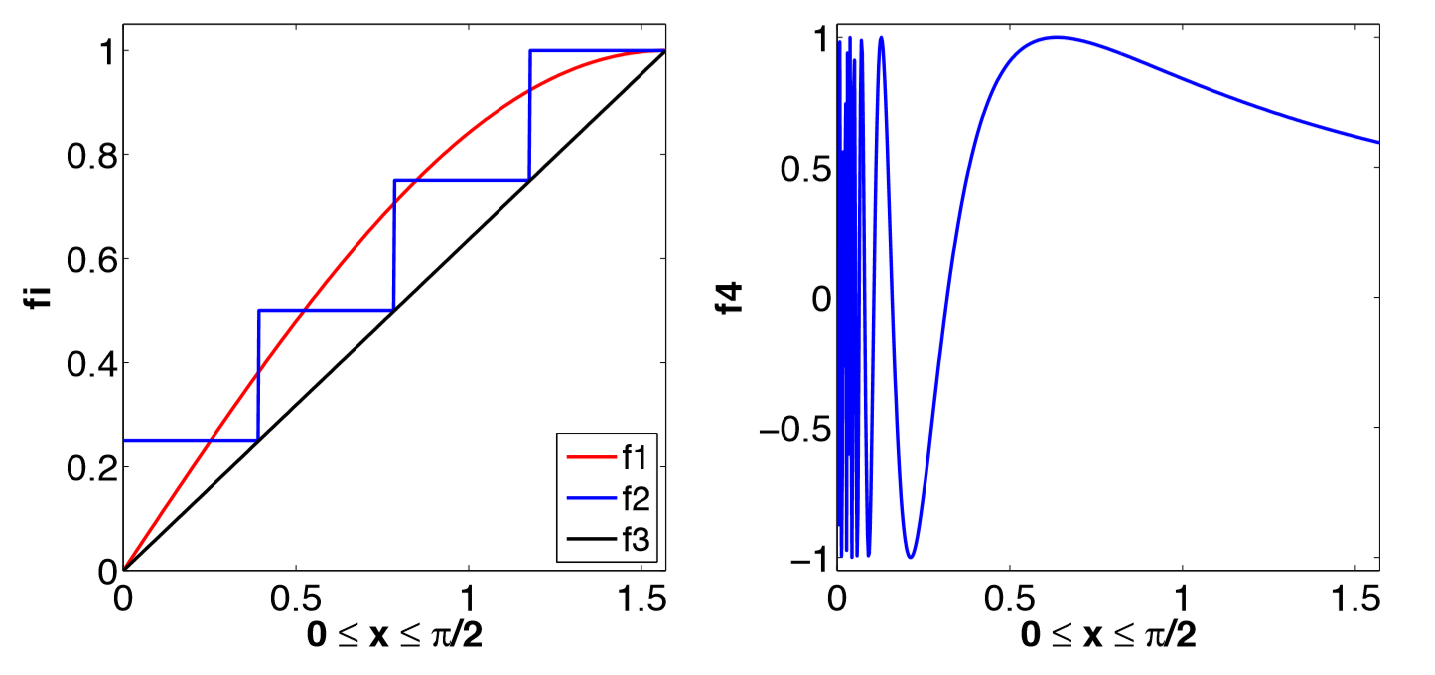
\includegraphics[width=0.8\linewidth]{image/boundary_condition/function_slove.png}
	\caption{(ซ้าย) ฟังก์ชันที่มีขอบเขตกับการแปรผันรวมที่มีค่าเดียวกัน (ขวา) ฟังก์ชันที่มีขอบเขตกับการแปรผันรวมอนันต์}
	\label{figure:sample-domain}
\end{figure}